% arara: pdflatex
% arara: indent
% arara: indent: {overwrite: yes}
% arara: indent: {output: jeopardy_Game2.tex}
% arara: indent: {silent: yes}
% arara: indent: {trace: yes}
% arara: indent: {localSettings: yes}
% arara: indent: {onlyDefault: on}
% arara: indent: { cruft: /home/camminady/.latexindent }

\documentclass{beamer}
\usepackage{tcolorbox}
\usepackage{ocgx}
\usepackage{graphicx}
\usepackage{commands}


\setbeamertemplate{navigation symbols}{}
\setbeamersize{text margin left=0cm, text margin right=0cm}
\tcbuselibrary{skins}

% Define the Categories here !!!!!!!
\def \firstcat {\textbf{Space}}
\def \secondcat {\textbf{Aachen}}
\def \thirdcat {\textbf{Code}}
\def \fourthcat {\textbf{The Force}}
\def \fifthcat {\textbf{Numbers}}

% Define the picture for the DOUBLE Bonus here !!!
\def \doublepic {
\includegraphics[scale=0.7]{../jeopardypics/Double_Jeopardy.png}}


%%%%%%%%%%%%%%%%%%%%%%%%%%%%%%%%%%%%%%%%%%%%%%%%%%%%%%%%%%%%%%%%%%%%%%%%%%%%%%%
%%%%%%%%%%%%%%%%%%%%%%%%%%%%%%%%%%%%%%%%%%%%%%%%%%%%%%%%%%%%%%%%%%%%%%%%%%%%%%%
\begin{document}
%%%%%%%%%%%%%%%%%%%%%%%%%%%%%%%%%%%%%%%%%%%%%%%%%%%%%%%%%%%%%%%%%%%%%%%%%%%%%%%

% Set up the HOME slide
\begin{frame}
    \hypertarget{home}{}
    \vspace*{-.5cm}
    \subjects{\firstcat}{\secondcat}{\thirdcat}{\fourthcat}{\fifthcat}
    \prizes
\end{frame}


%%%%%%%%%%%%%%%%%%%%%%%%%%%%%%%%%%%%%%%%%%%%%%%%%%%%%%%%%%%%%%%%%%%%%%%%%%%%%
% Category 1
%%%%%%%%%%%%%%%%%%%%%%%%%%%%%%%%%%%%%%%%%%%%%%%%%%%%%%%%%%%%%%%%%%%%%%%%%%%%%
\content                       
{s1-100}                     
{\firstcat}                          
{100}{    
	\begin{textarea}[]
		\only<1>{
			After Armstrong, this man was the second person to walk on the moon.
		}
		\only<2>{
			Who is Buzz Aldrin?
		}
	\end{textarea}   
}


\content                       
{s1-200}                     
{\firstcat}                          
{200}{    
	\begin{textarea}[]
		\only<1>{
			\begin{columns}[c]
				\column{.3\textwidth}
				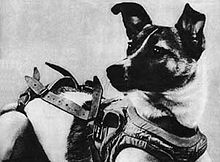
\includegraphics[height=1.0\linewidth]{../categories/media/space/laika.jpg}
				\column{.3\textwidth}	
				This soviet dog became one of the first animals in space.
			\end{columns}
			
		}
		\only<2>{
			Who is Laika?
		}
	\end{textarea}           
}


\content           
{s1-300}                     
{\firstcat}                          
{300}{                       
	\begin{textarea}[]
		\only<1>{
			\begin{columns}[c]
				\column{.3\textwidth}
				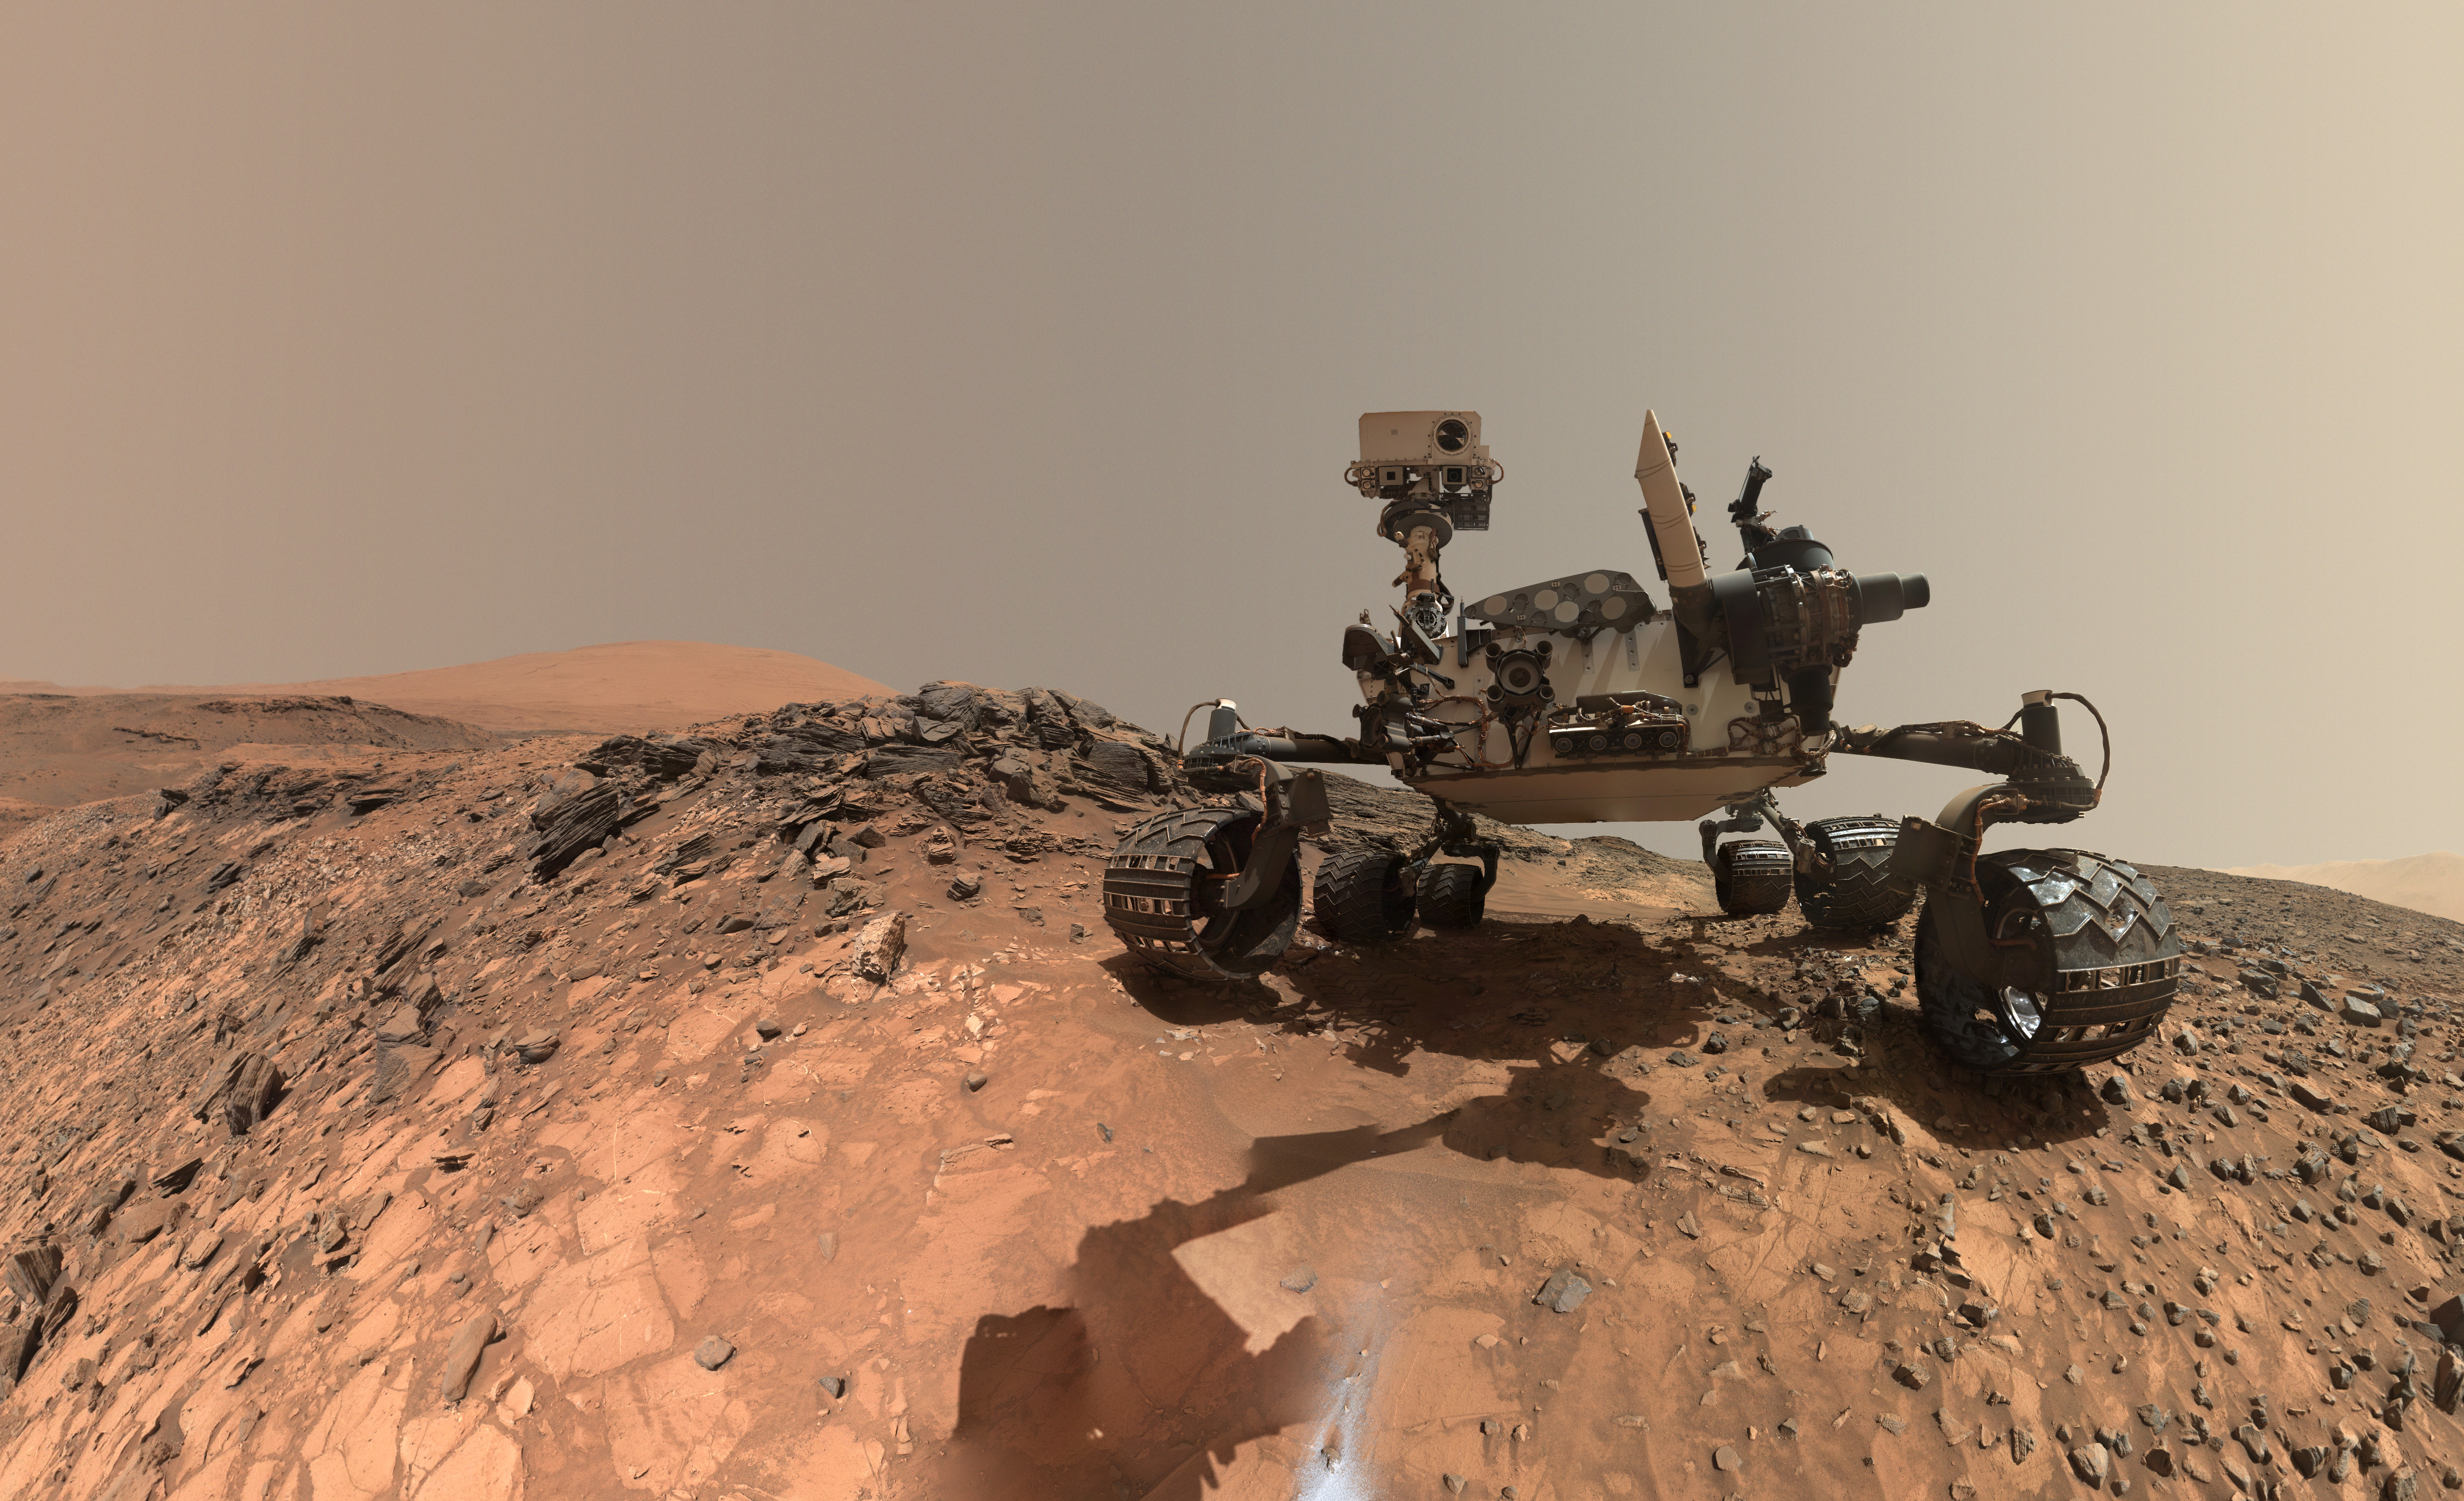
\includegraphics[height=.7\linewidth]{../categories/media/space/selfie.jpg}
				\column{.3\textwidth}	
				It took quite some effort to take a selfie of this guy.
			\end{columns}
		}
		\only<2>{
			What is the Curiosity Rover?
		}
	\end{textarea}
}


\content                       
{s1-400}                     
{\firstcat}                          
{400}{    
	\begin{textarea}[]
		\only<1>{
			In 2003, this space shuttle reentry ended in a disaster due to parts of the insulation breaking off.
		}
		\only<2>{
			What is the Space Shuttle Columbia?
		}
	\end{textarea}   
}


\content                       
{s1-500}                     
{\firstcat}                          
{500}{    
	\begin{textarea}[]
		\only<1>{
			Founded by the Tesla Motors CEO, this company achieved the first vertical landing of a first stage.
		}
		\only<2>{
			What is SpaceX?
		}
	\end{textarea}
}


%%%%%%%%%%%%%%%%%%%%%%%%%%%%%%%%%%%%%%%%%%%%%%%%%%%%%%%%%%%%%%%%%%%%%%%%%%%%%%%
% Category 2
%%%%%%%%%%%%%%%%%%%%%%%%%%%%%%%%%%%%%%%%%%%%%%%%%%%%%%%%%%%%%%%%%%%%%%%%%%%%%%%

%%%%%%%%%%%%%%%%%%%%%%%%%%%%%%%%%%%%%%%%%%%%%%%%%%%%%%%%%%%%%%%%%%%%%%%%%%%%%%%
% Category 2
%%%%%%%%%%%%%%%%%%%%%%%%%%%%%%%%%%%%%%%%%%%%%%%%%%%%%%%%%%%%%%%%%%%%%%%%%%%%%%%

%%%%%%%%%%%%%%%%%%%%%%%%%%%%%%%%%%%%%%%%%%%%%%%%%%%%%%%%%%%%%%%%%%%%%%%%%%%%%%%
% Category 2
%%%%%%%%%%%%%%%%%%%%%%%%%%%%%%%%%%%%%%%%%%%%%%%%%%%%%%%%%%%%%%%%%%%%%%%%%%%%%%%
%%%%%%%%%%%%%%%%%%%%%%%%%%%%%%%%%%%%%%%%%%%%%%%%%%%%%%%%%%%%%%%%%%%%%%%%%%%%%%%
% Category 2
%%%%%%%%%%%%%%%%%%%%%%%%%%%%%%%%%%%%%%%%%%%%%%%%%%%%%%%%%%%%%%%%%%%%%%%%%%%%%%%

\end{document}
